\chapter{Method}
This chapter outlines each test case, describes the motivation behind the test plan, and delves into both the hardware and software design required to implement the methodology. 

The overall test principle was derived from traditional sensorimotor synchronization tasks in which a user is asked to tap to a corresponding stimulus. The time delta between the tap onset and the stimulus onset is tracked and plotted for future analysis. Since the haptic domain is of primary focus, the auditory modality functions primarily as a benchmark or baseline foundation.  The work presented in \ref{visualMet} extensively covers the idea of the interstitial beat occupying the visual domain and as such will not be re-evaluated here.

\todo{Fill method intro in with more detail}

Each test case is defined and presented in \ref{testPlan}. The overall software development is detailed in \ref{development}. The hardware setup and code re-purposing from TapArduino is discussed in \ref{tap_arduino}.

\section{Test Plan} \label{testPlan}
Testing was divided into two major sections, \textbf{Steady} and \textbf{Dynamic}, implying either an \textit{isochronous} beat or a \textit{non-isochronous} pulse respectively. While structurally identical, the dynamic tests however focussed on rubato within a range starting at the predefined BPM and rising or falling within a specified window. The chosen tempi parallels slow walking to running gaits spanning a range of 45-180 beats per minute.

Each section had three subsections centered around either an audible metronome tone (\textbf{A1, A3}), musical note (\textbf{A2, A4}), and lastly the haptic modality (\textbf{H1, H2}). Subsections were further broken down into \textbf{a} and \textbf{b} sections, denoting either \textit{discrete} or \textit{interstitial}/\textit{continuous} mode of operation. A breakdown of the test plan is shown in Figure \ref{fig:TestPlan}.

As discussed in Chapter 3, the haptic was designed with two operating modes in mind, discrete and continuous. These modes were programmatically controlled to match the desired test cases, extensively explained in section \ref{development}
\begin{table}[]
    \centering
    \resizebox{\textwidth}{!}{%
    \begin{tabular}{cclllcclll}
    \hline
    \multicolumn{10}{c}{Steady} \\ \hline
    \multicolumn{3}{c}{Discrete} & BPM & Runtime (sec) & \multicolumn{3}{c}{Interstitial} & BPM & Runtime (sec) \\
    \multirow{4}{*}{A1a} & \multirow{4}{*}{click} & i. & 45 & 20 & \multirow{4}{*}{A1b} & \multirow{4}{*}{legato chime (swing click)} & i. & 45 & 30 \\
     &  & ii. & 90 & 20 &  &  & ii. & 90 & 16 \\
     &  & iii. & 135 & 20 &  &  & iii. & 135 & 11 \\
     &  & iv. & 180 & 20 &  &  & iv. & 180 & 8 \\
    \multirow{4}{*}{A2a} & \multirow{4}{*}{staccato music (melody)} & i. & 45 & 32 & \multirow{4}{*}{A2b} & \multirow{4}{*}{legato music (melody)} & i. & 45 & 32 \\
     &  & ii. & 90 & 16 &  &  & ii. & 90 & 16 \\
     &  & iii. & 135 & 11 &  &  & iii. & 135 & 11 \\
     &  & iv. & 180 & 8 &  &  & iv. & 180 & 8 \\
    \multirow{4}{*}{H1a} & \multirow{4}{*}{poke / all on (instantaneous)} & i. & 45 & 15 & \multirow{4}{*}{H1b} & \multirow{4}{*}{oscillate down and back up} & i. & 45 & 15 \\
     &  & ii. & 90 & 15 &  &  & ii. & 90 & 15 \\
     &  & iii. & 135 & 15 &  &  & iii. & 135 & 15 \\
     &  & iv. & 180 & 15 &  &  & iv. & 180 & 15 \\ \hline
    \multicolumn{10}{c}{Dynamic} \\ \hline
    \multicolumn{3}{c}{Discrete} & BPM & Runtime (sec) & \multicolumn{3}{c}{Interstitial} & BPM & Runtime (sec) \\
    \multirow{4}{*}{A3a} & \multirow{4}{*}{click} & i. & 45 +/- 15 & 20 & \multirow{4}{*}{A3b} & \multirow{4}{*}{legato chime (swing click)} & i. & 45 +/- 15 & 20 \\
     &  & ii. & 90 +/- 15 & 10 &  &  & ii. & 90 +/- 15 & 10 \\
     &  & iii. & 135 +/- 15 & 10 &  &  & iii. & 135 +/- 15 & 10 \\
     &  & iv. & 180 +/- 15 & 10 &  &  & iv. & 180 +/- 15 & 10 \\
    \multirow{4}{*}{A4a} & \multirow{4}{*}{staccato music (melody)} & i. & 45 +/- 15 & 30 & \multirow{4}{*}{A4b} & \multirow{4}{*}{legato music (melody)} & i. & 45 +/- 15 & 30 \\
     &  & ii. & 90 +/- 15 & 15 &  &  & ii. & 90 +/- 15 & 15 \\
     &  & iii. & 135 +/- 15 & 10 &  &  & iii. & 135 +/- 15 & 10 \\
     &  & iv. & 180 +/- 15 & 10 &  &  & iv. & 180 +/- 15 & 10 \\
    \multirow{4}{*}{H2a} & \multirow{4}{*}{poke / all on (instantaneous)} & i. & 45 +/- 10 & 15 & \multirow{4}{*}{H2b} & \multirow{4}{*}{oscillate down and back up} & i. & 45 +/- 10 & 15 \\
     &  & ii. & 90 +/- 5 & 15 &  &  & ii. & 90 +/- 5 & 15 \\
     &  & iii. & 135 +/- 3 & 15 &  &  & iii. & 135 +/- 3 & 15 \\
     &  & iv. & 180 +/- 1 & 15 &  &  & iv. & 180 +/- 1 & 15
    \end{tabular}%
    }
    \caption{Test Plan}
    \label{fig:TestPlan}
\end{table}

\subsection{Audio File Generation}
All tracks were rendered using the digital audio workstation (DAW) \textit{Logic Pro X} as \textit{.wav} files at a 44.1kHz sample rate with 16 bit resolution.
\subsubsection{Metronomic click and legato chime}
\begin{wrapfigure}[8]{r}{5cm}
    \centering
    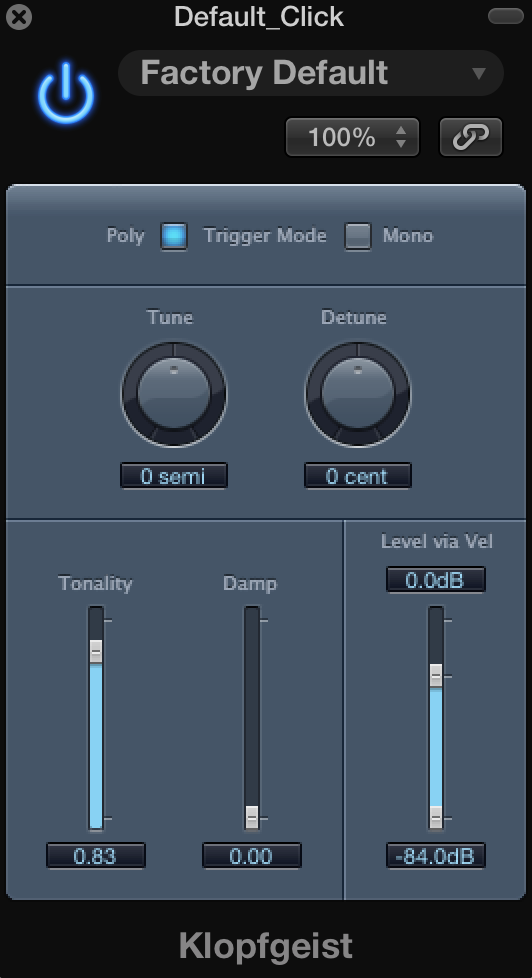
\includegraphics[width=0.25\textwidth]{klopfgeist}
    \caption{Default metronome}
    \label{fig:klopfgeist}
\end{wrapfigure}
\textbf{A1a} and \textbf{A3a} required a standard metronomic pulse. This was accomplished using the default Klopfgeist (metronome) plugin from Logic Pro X. No additional tuning was modified and the tonality was left at 0.83 of unity as shown in \ref{fig:klopfgeist}. 

\textbf{A1b} and \textbf{A3b} however required a swing or legato type of chime in order to convey filling the interstitial space. To capture this effect the Klopfgeist tonality was increased to unity and tuned -27 semitones lower which served to both soften diminish the discrete click, provided an elongated or continuous audible sensation. To give the impression of a sound that was ramping up in amplitude and decaying after the peak, a tremolo effect which mimics a sawtooth wave was added to the signal chain as seen in \ref{fig:modClick}. Last, a multi-band EQ was placed at the end of the signal chain with a bandpass filter from 95Hz-750Hz to remove unwanted frequency presence and a 3.5dB high-Q peak at 220Hz to emphasize the tonality.

\begin{figure}[H]
    \centering
    \caption{Modified click parameters for interstitial tests.}
        \subfloat[Modified metronome]{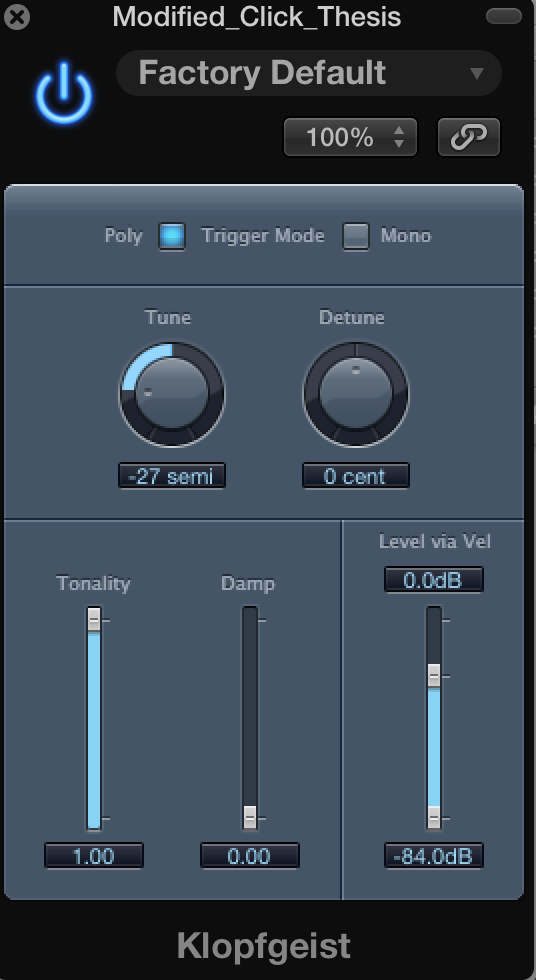
\includegraphics[width=0.25\columnwidth]{Klopfgeist_Modified}}
        \qquad
        \subfloat[Superimposed tremolo]{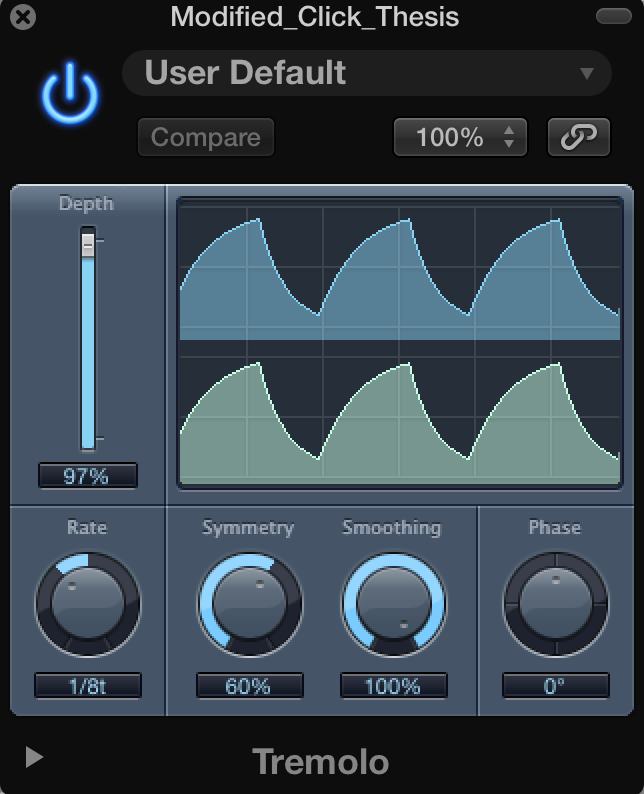
\includegraphics[width=0.4\columnwidth]{Tremolo}}
        \qquad
        \subfloat[Equalized tone]{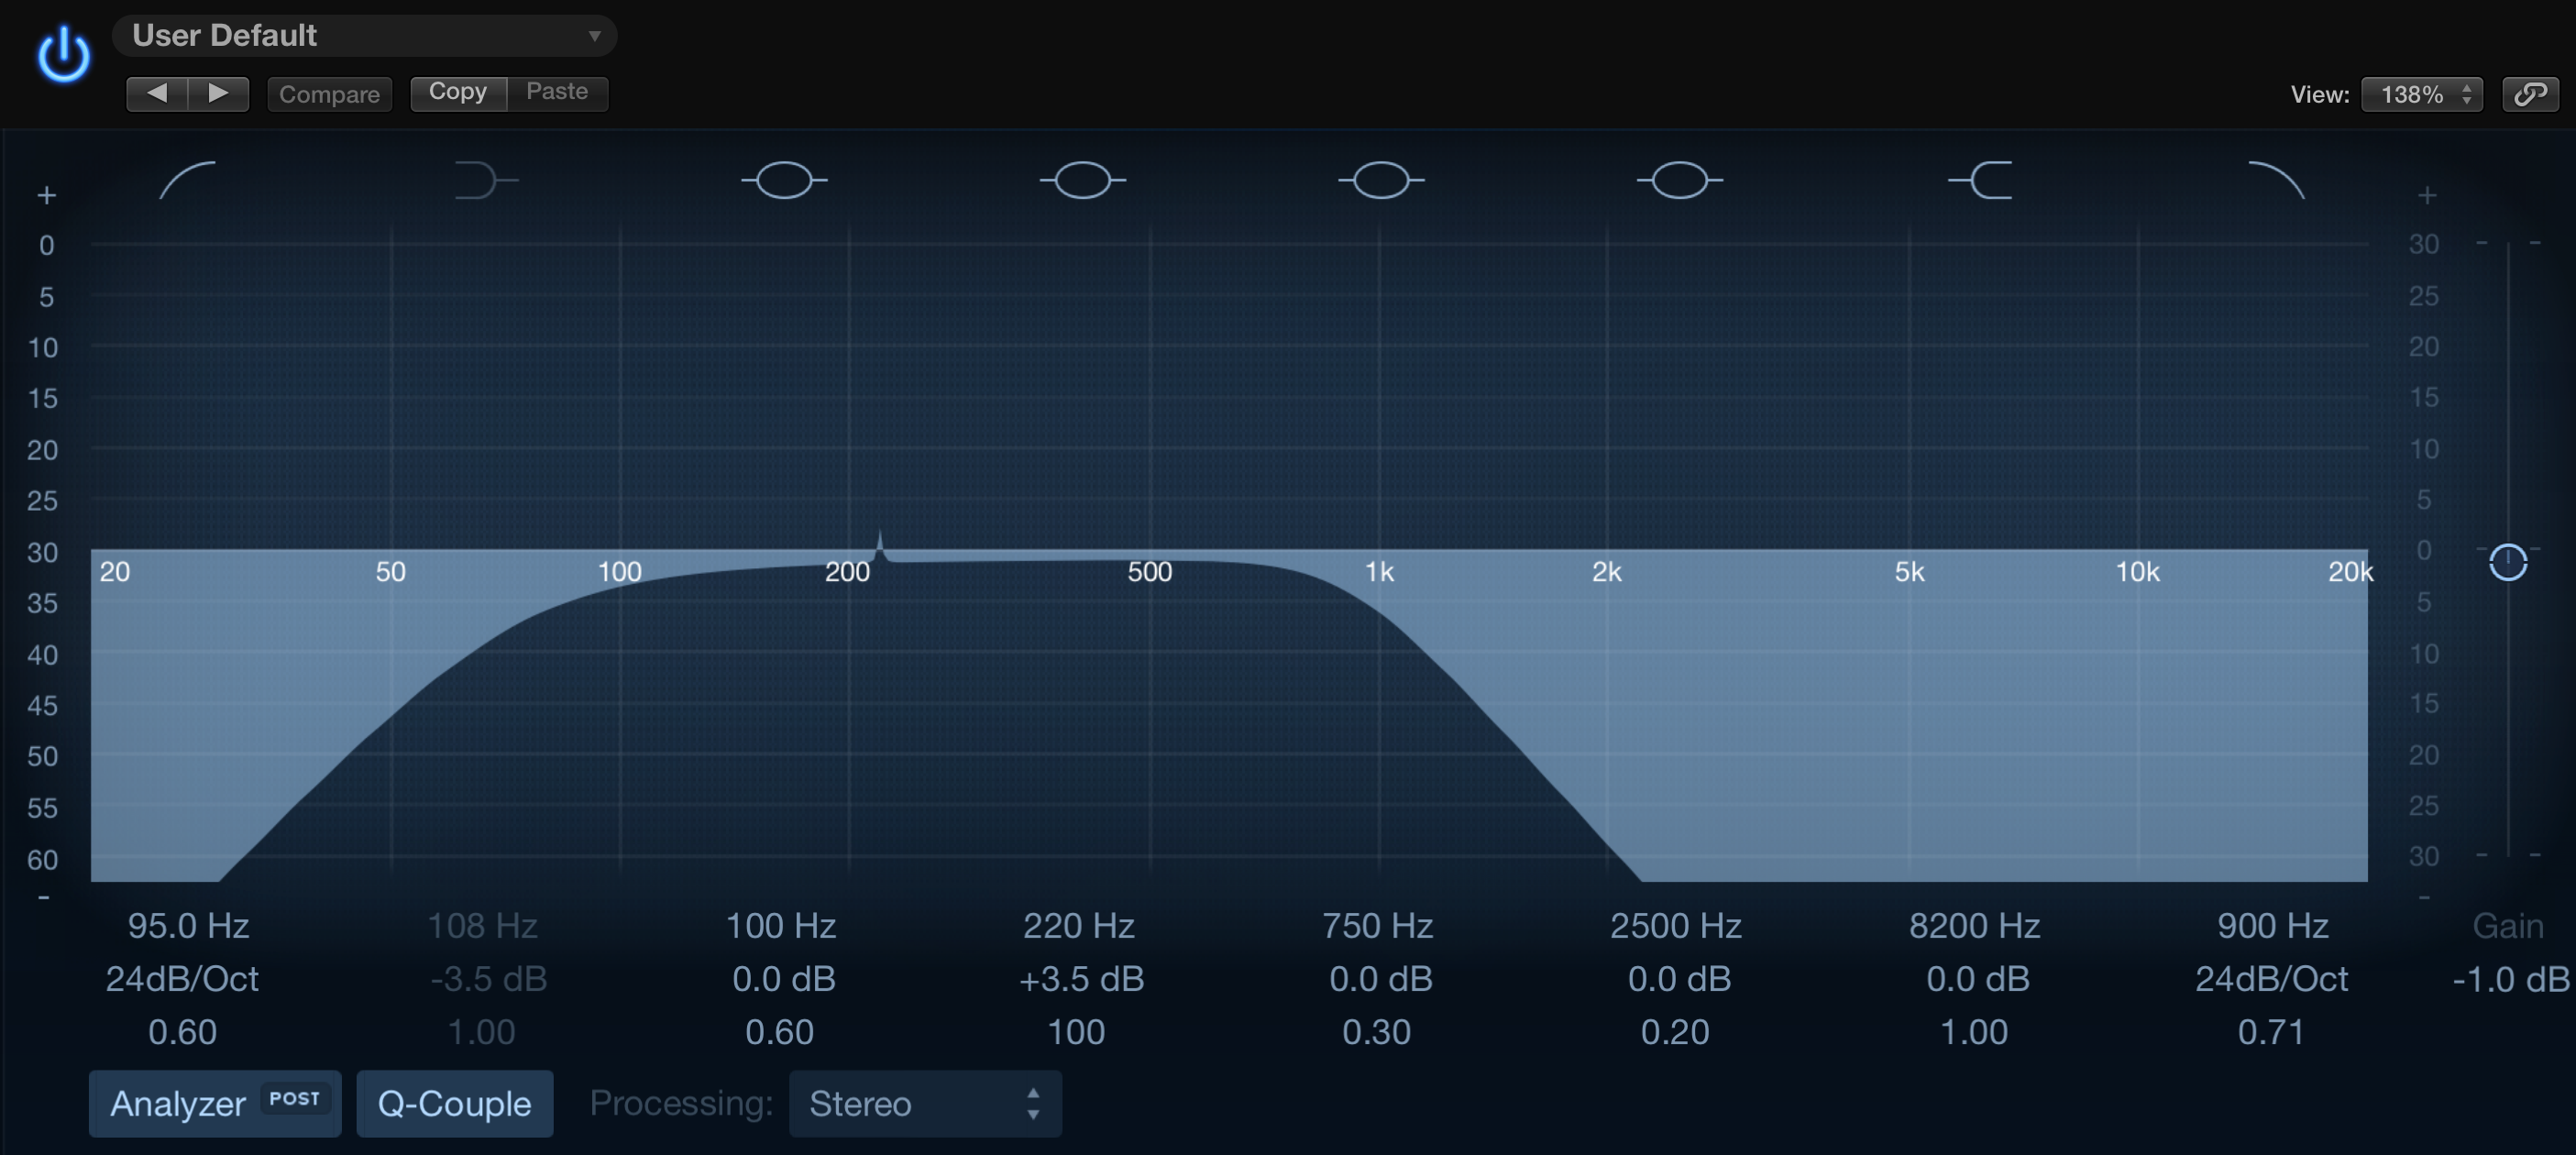
\includegraphics[width=\textwidth,height=0.25\textheight]{Modified_Click_EQ}}
    \label{fig:modClick}
\end{figure}

The resultant waveform encapsulated the occupation of the interstitial space. A comparison of this waveform in contrast to it's discrete counterpart is shown in \ref{fig:click_comparison}. Note the envelope of signal (b) follows a natural build up and decay.

\begin{figure}[H]
    \centering
    \caption{Metronomic waveform comparison}
        \subfloat[A3a1: discrete audible click]{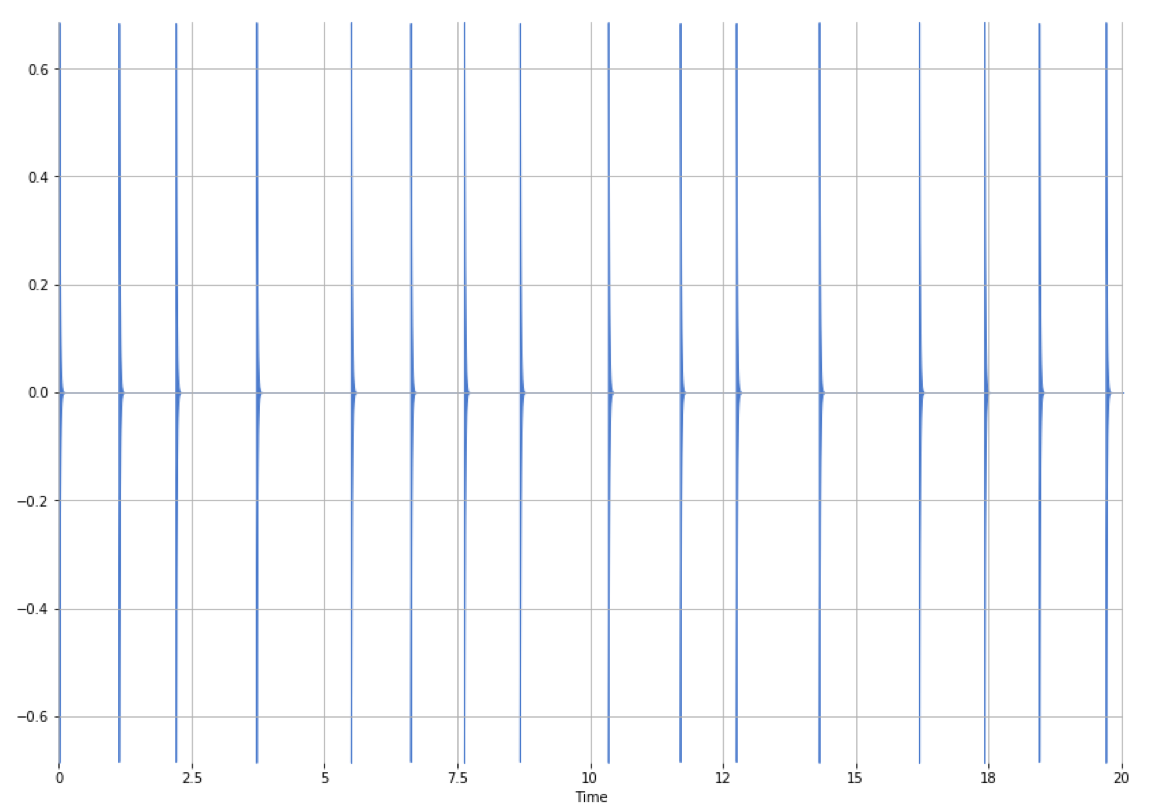
\includegraphics[width=0.5\columnwidth]{Click_waveform}}
        \subfloat[A3b1: interstitial tone]{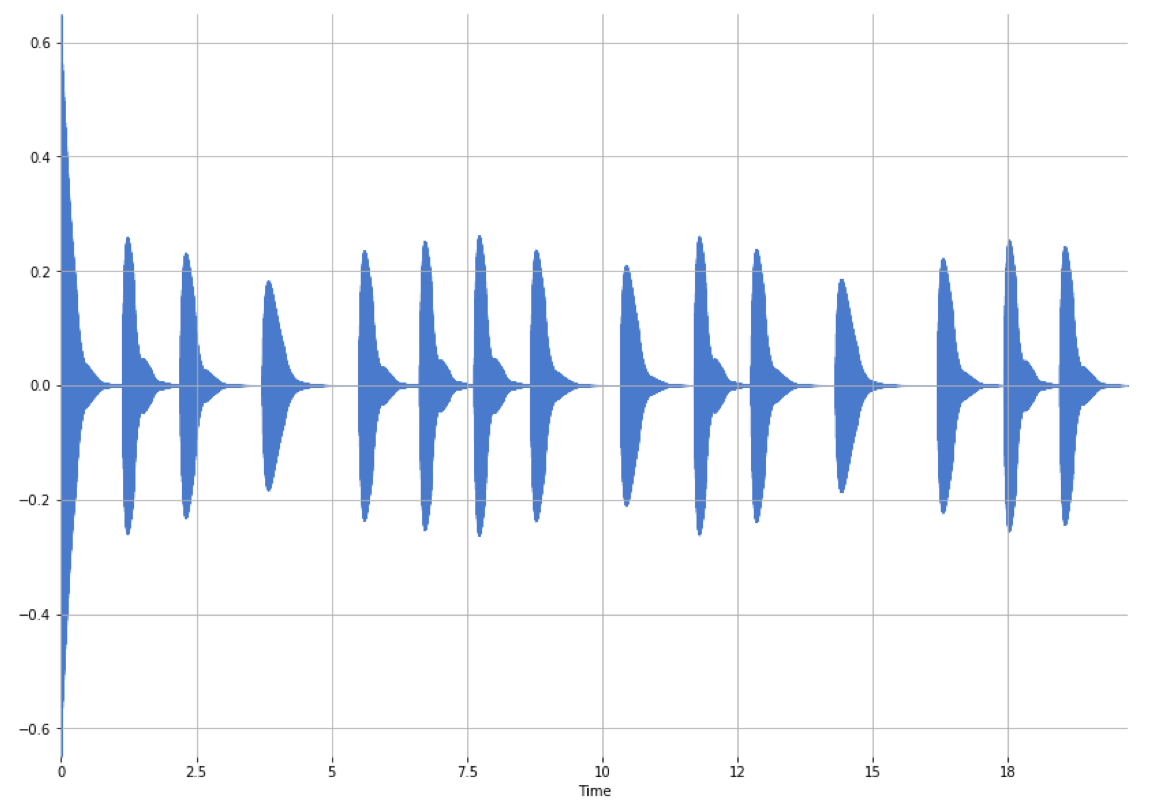
\includegraphics[width=0.5\columnwidth]{SwingClick_waveform}}
    \label{fig:click_comparison}
\end{figure}

\subsubsection{Stacatto and legato melody}
As a specific musical listening task, test cases \textbf{A2a}, \textbf{A4a} and \textbf{A2b}, \textbf{A4b} involve synchronization to a simple melodic sequence of notes. The music chosen was the nursery rhyme \textit{Pat-A-Cake}. The initial mockup was drafted in Sibelius and exported to Logic Pro X for bpm adjustment.

\todo{Expand the reasoning for the musical tests}

Each quarter note represents a beat and therefore a tap onset. In order to emphasize a discrete event for test cases \textbf{A2a} and \textbf{A4a}, notes were input as stacatto, shown below: \ref{fig:pat-a-cake_a2a}.

\begin{figure}[H]
    \centering
    \includegraphics[width=\textwidth]{Pat-a-Cake_a2a}
    \label{fig:pat-a-cake_a2a}
\end{figure}

The interstitial counterpart of these test cases (\textbf{A2b}, \textbf{A4b}) underwent crescendo and decrescendo after every note onset with forte notes surrounded by mezzopiano to give the impression of amplitude build up and decay, shown below: \ref{fig:pat-a-cake_a2b} 

\begin{figure}[H]
    \centering
    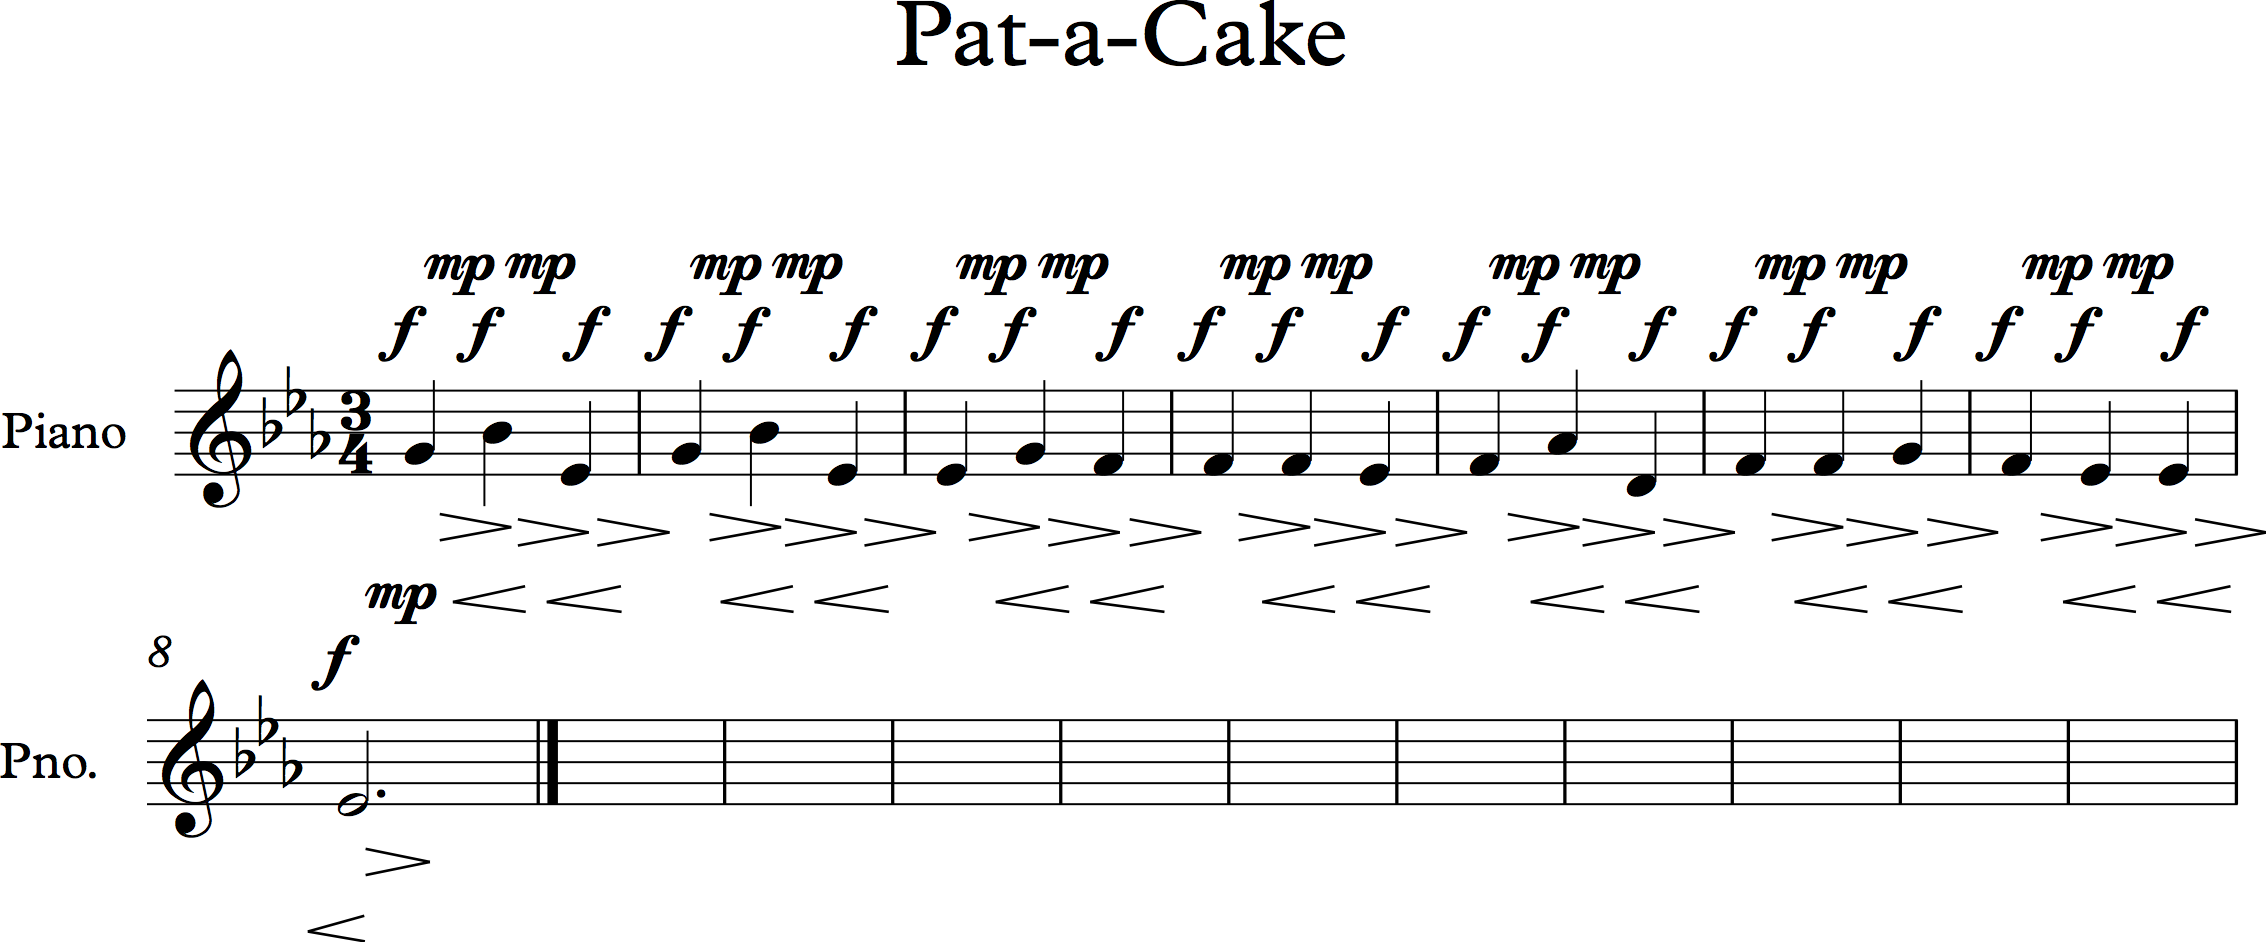
\includegraphics[width=\textwidth]{Pat-a-Cake_A2b}
    \label{fig:pat-a-cake_a2b}
\end{figure}

Note below in \ref{fig:music_comparison} the gradual, nearly exponential decay displayed in the interstitial tone as a result of the legato input.

\begin{figure}[H]
    \centering
    \caption{Musical waveform comparison}
        \subfloat[A2a1: stacatto melody]{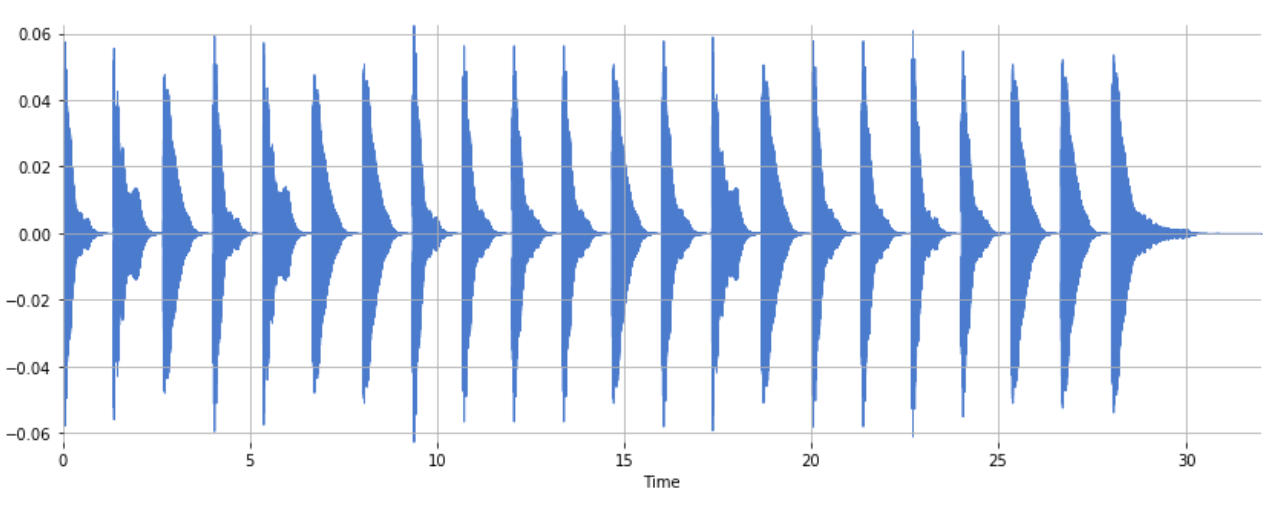
\includegraphics[width=\columnwidth]{A2a1_waveform}}
        \qquad
        \subfloat[A2b1: legato melody]{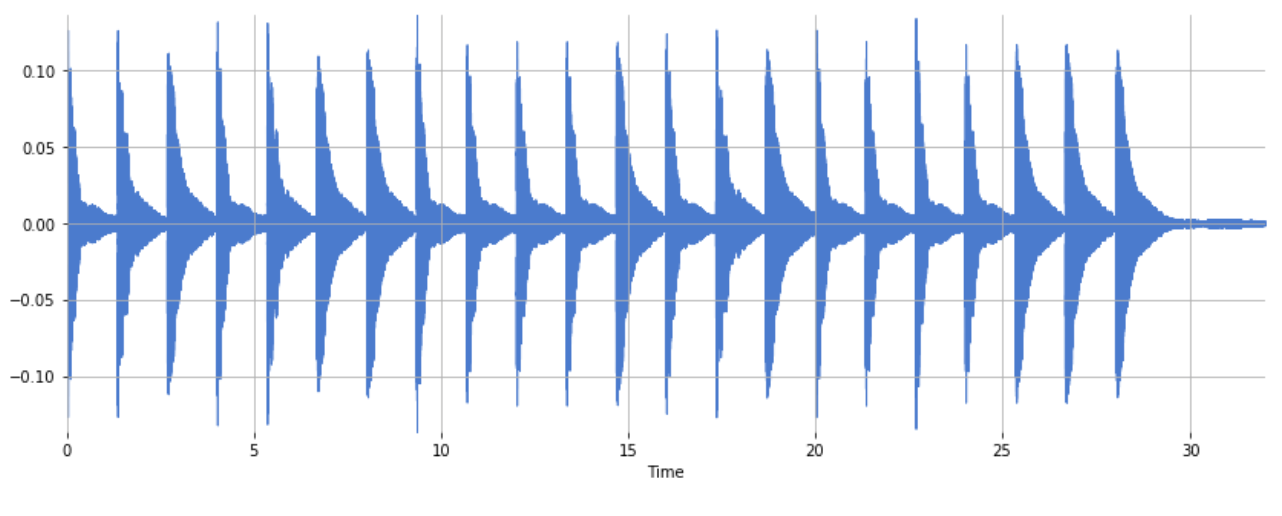
\includegraphics[width=\columnwidth]{A2b1_waveform}}
    \label{fig:music_comparison}
\end{figure}

\subsubsection{Dynamic tempi manipulation - audio}
Dynamic manipulation of tempo was accomplished in \textit{Logic Pro X} through automation of the tempo parameter over the time period of the desired waveform. Each test case started on one of the pre-defined BPM's (45, 90, 135, 180) but traversed either sinusoidally or triangularly through time as peaks and troughs ranging plus or minus 15 bpm; shown in \ref{fig:dynamic_audio}.

\begin{figure}[H]
    \centering
    \caption{Dynamic audio tempo automation patterns}
        \subfloat[45 +/- 15]{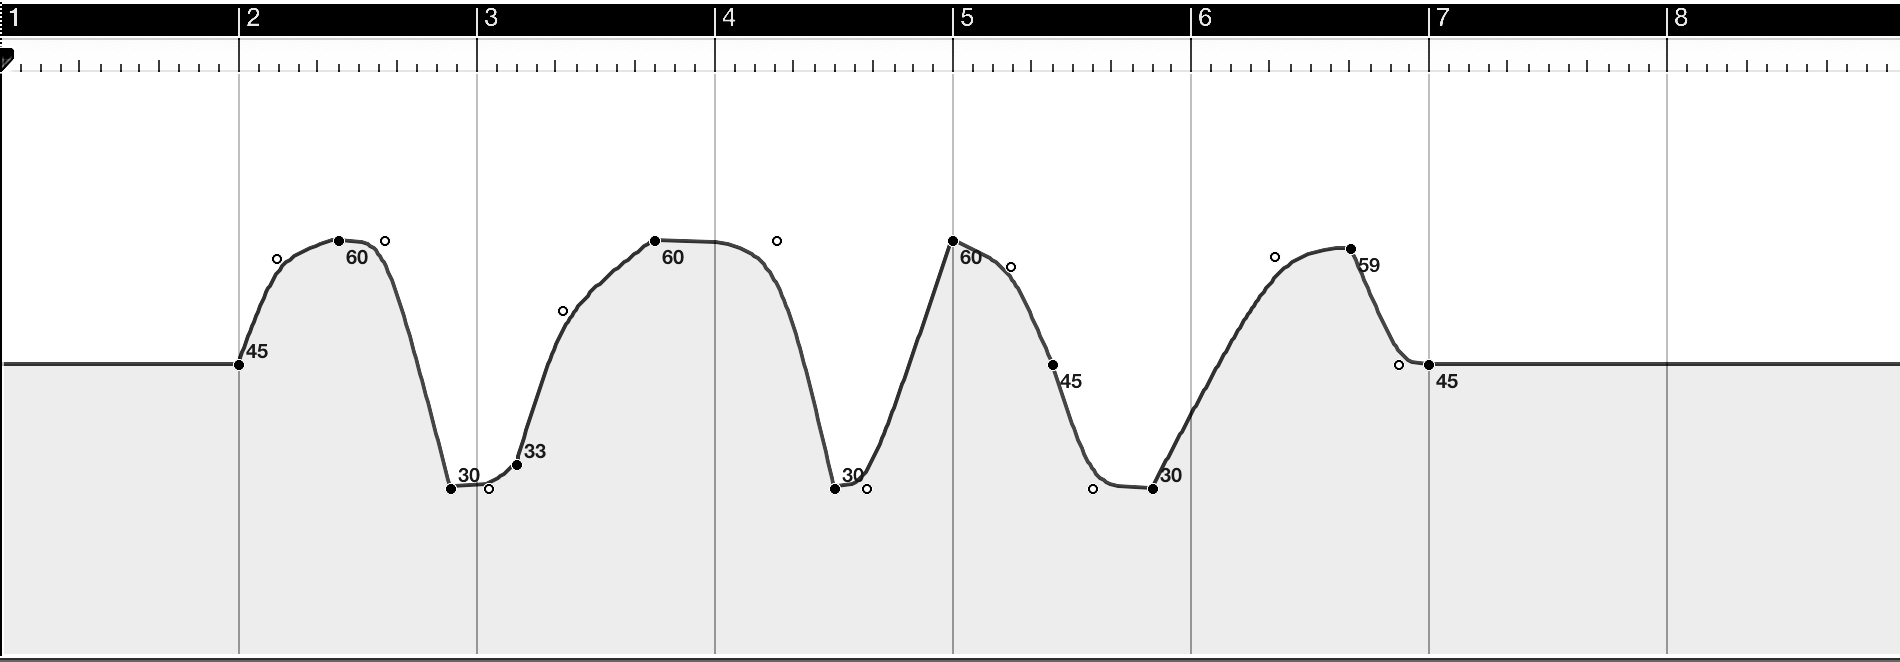
\includegraphics[width=.5\columnwidth]{dynamic_45}}
        \subfloat[90 +/- 15]{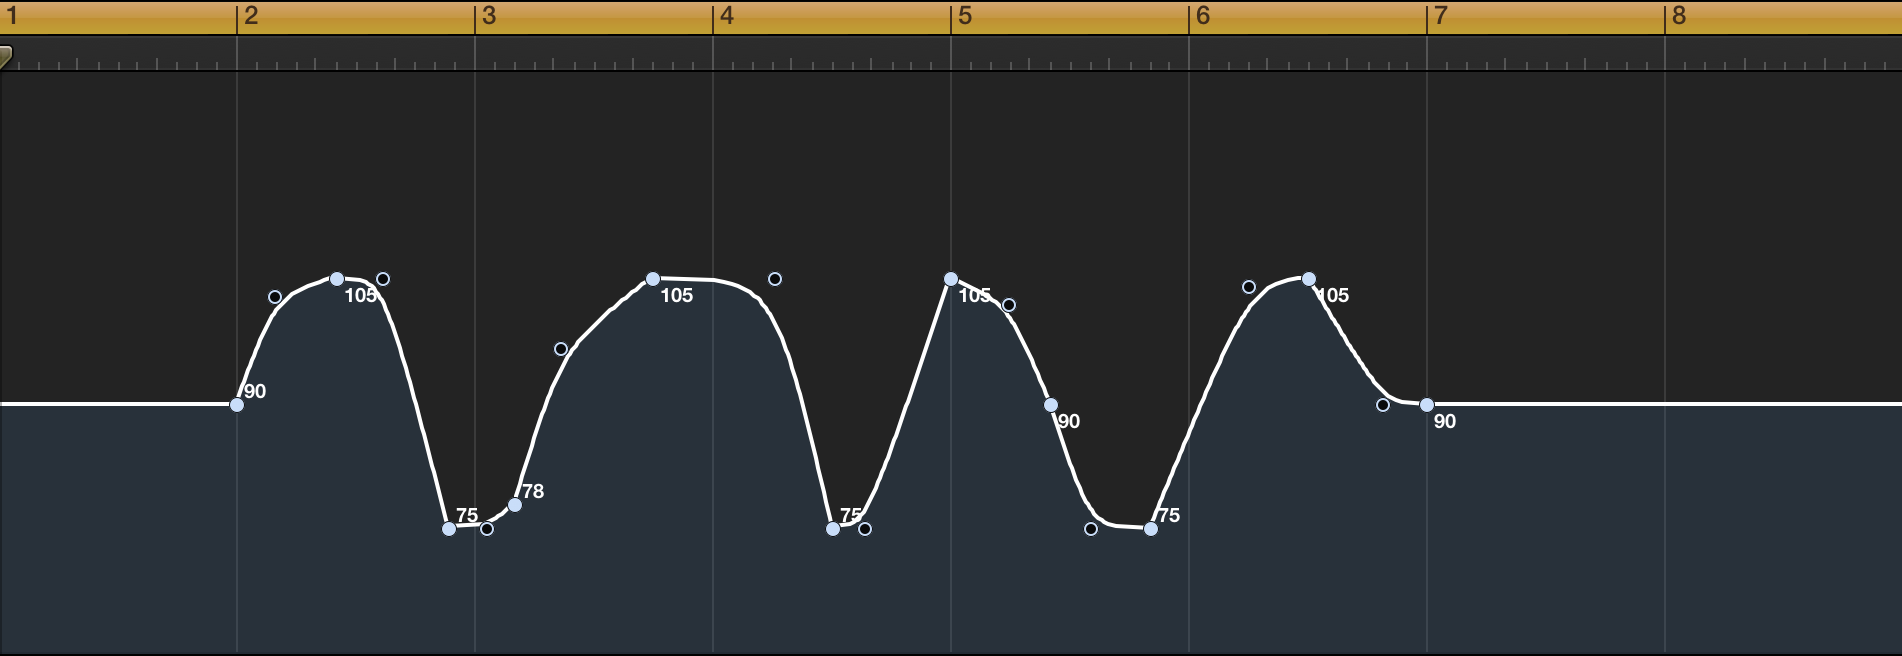
\includegraphics[width=.5\columnwidth]{dynamic_90}}
        \qquad
        \subfloat[135 +/- 15]{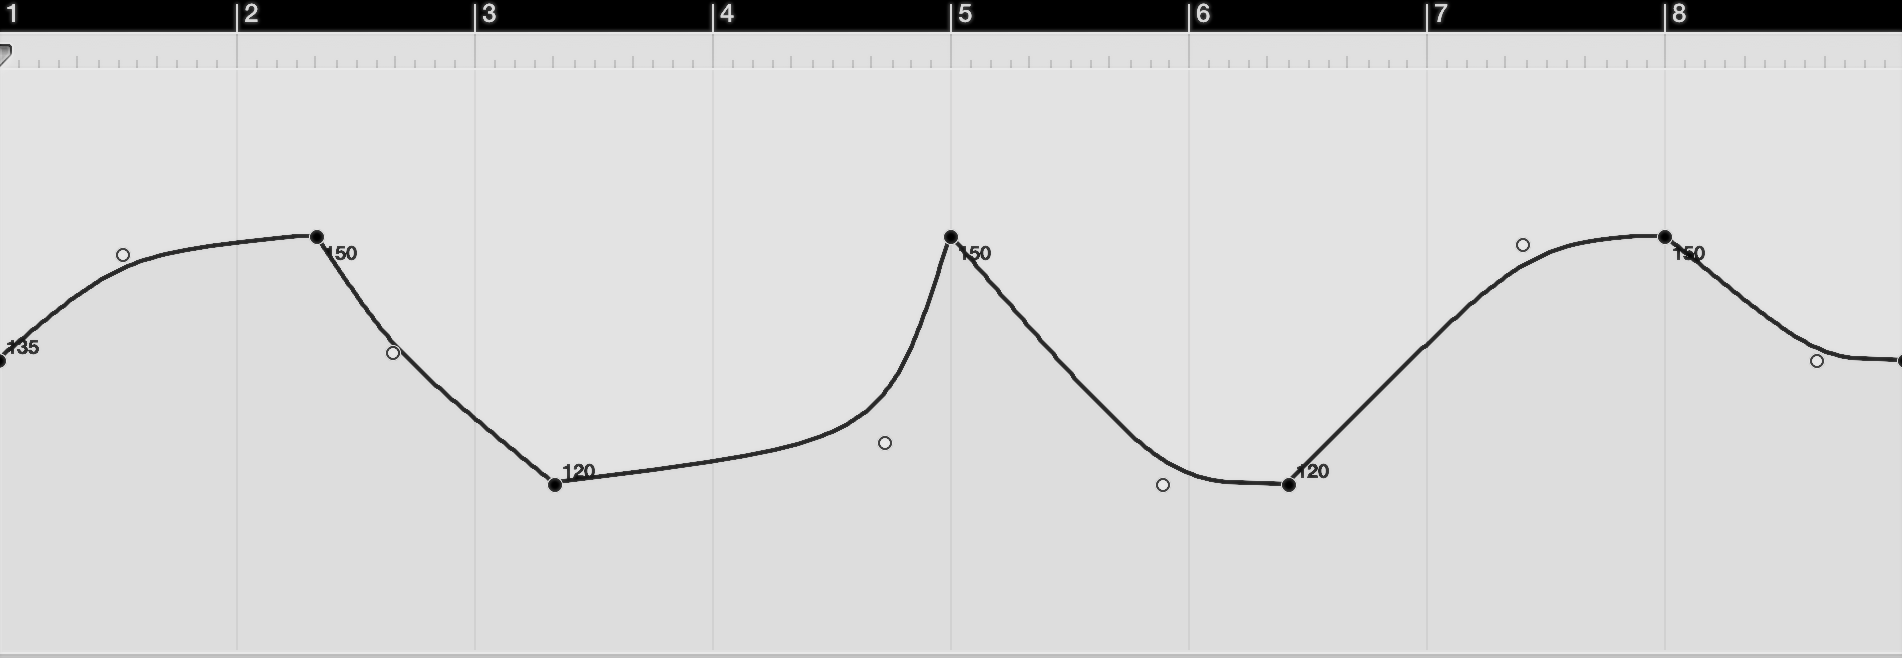
\includegraphics[width=.5\columnwidth]{dynamic_135}}
        \subfloat[180 +/- 15]{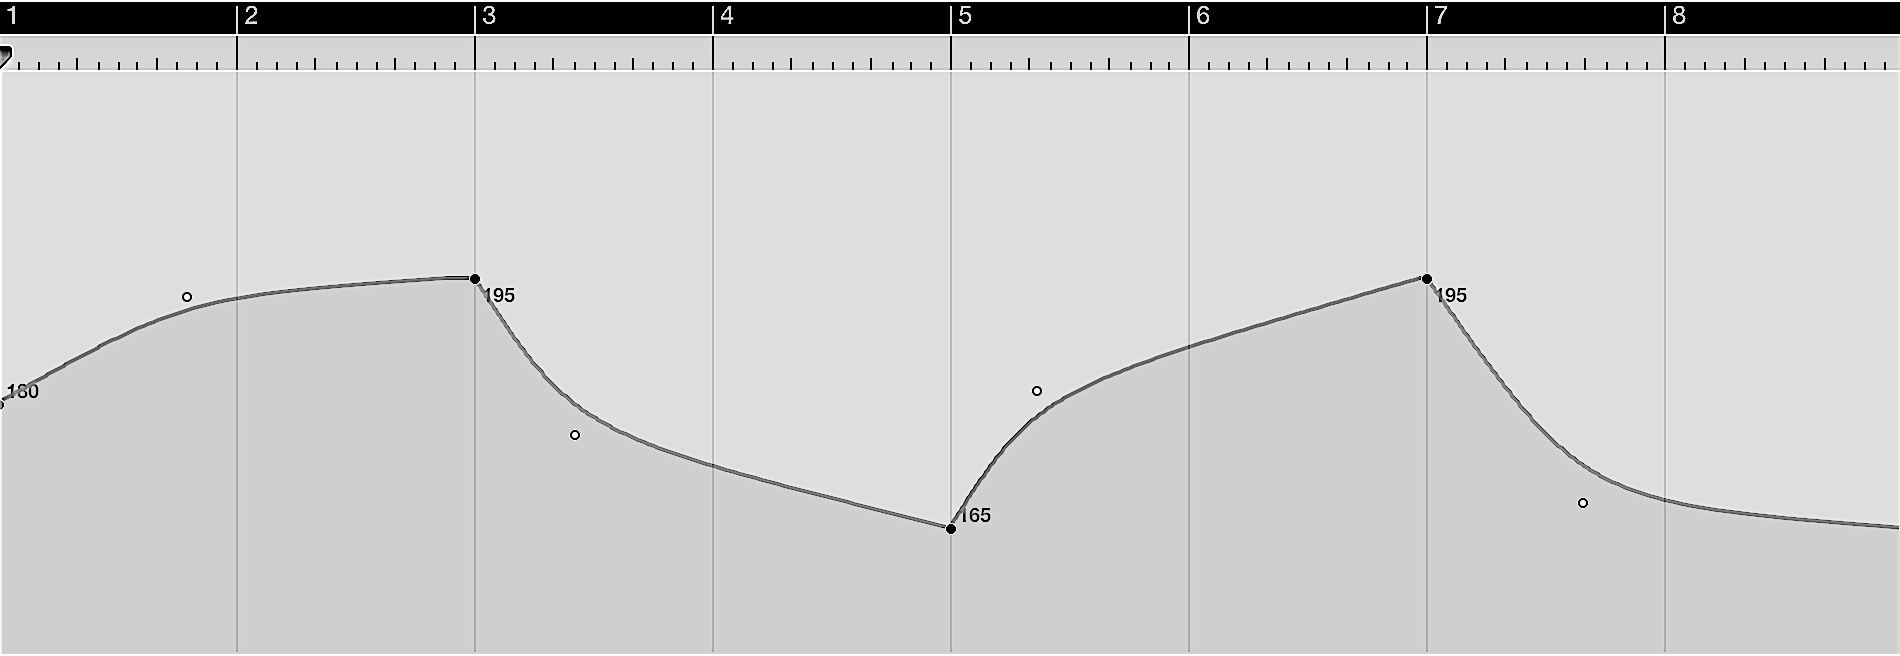
\includegraphics[width=.5\columnwidth]{dynamic_180}}
    \label{fig:dynamic_audio}
\end{figure}

\section{Test Suite}
High precision data acquisition and the minimization of delay were the central foci of the test suite design. Due to the extensive amount of publicly available libraries, multithreading capability, and plot integration via matplotlib, \textit{Python} was chosen as the development environment. Complementary to the software platform was the implementation of a tap onset detection mechanism via force sensitive resistor (FSR) and the \textit{Arduino Uno}. 

\subsection{Software Development} \label{development}
            Discuss code breakdown
            
            GUI
            
            Haptic onset detection
            
            Tap onset detection
            
            Multithreading
            
            Audio onset detection
            
            Plotting

\subsection{Tap Onset Hardware}    \label{tap_arduino}
\subsubsection{Tap Onset Latency Evaluation}

A sensorimotor synchronization experiment was conducted to discover how auditory feedback to a tap onset could be presented with minimal latency and responses recorded with the most accuracy. It was found that not only was the auditory response latency the least for the Arduino system using a force sensitive resistor (mean = 0.6 ms, sd = 0.3), but it had missed the fewest taps and recorded the least superfluous responses as compared to a percussion pad with the FTAP and Max MSP systems [Tap Arduino, 1].

\subsection{Delay Evaluation} \label{latencyCalc}

Overall strategy to minimize delay maximize accuracy/precision

Sources of potential error:

    *FTDI/USB -> Pro Trinket (16MHz) --> Laptop

    *USB -> Arduino -> Laptop

    *Serial write to haptic to motor spin up

    *FSR analog read/mentioned debounce

    Sol: python threading

    Evaluation with scope:

\subsection{Setup} \label{testSetup}

To initialize setup, the user is seated and given a pair of closed-back headphones. The FSR is situated to their preference, either dominant or non-dominant hand, and secured into place. Unlike a keyboard or button the FSR gives no feedback or rebound;psychologically ensuring a confident tap on each onset while providing no tactile response. This approach avoids intrinsic lag as there are no mechanical components involved. The delay limit is defined by the threshold applied in the software to avoid debounce, as discussed in Section \ref{}

The user will input their name, read the instructions, agree to the conditions of the test suite, and commence with the test. The order every user encounters will differ as the tests are scrambled. Upon completion, the users are asked to fill out a survey and the results are displayed.

\begin{figure}[H]
    \centering
    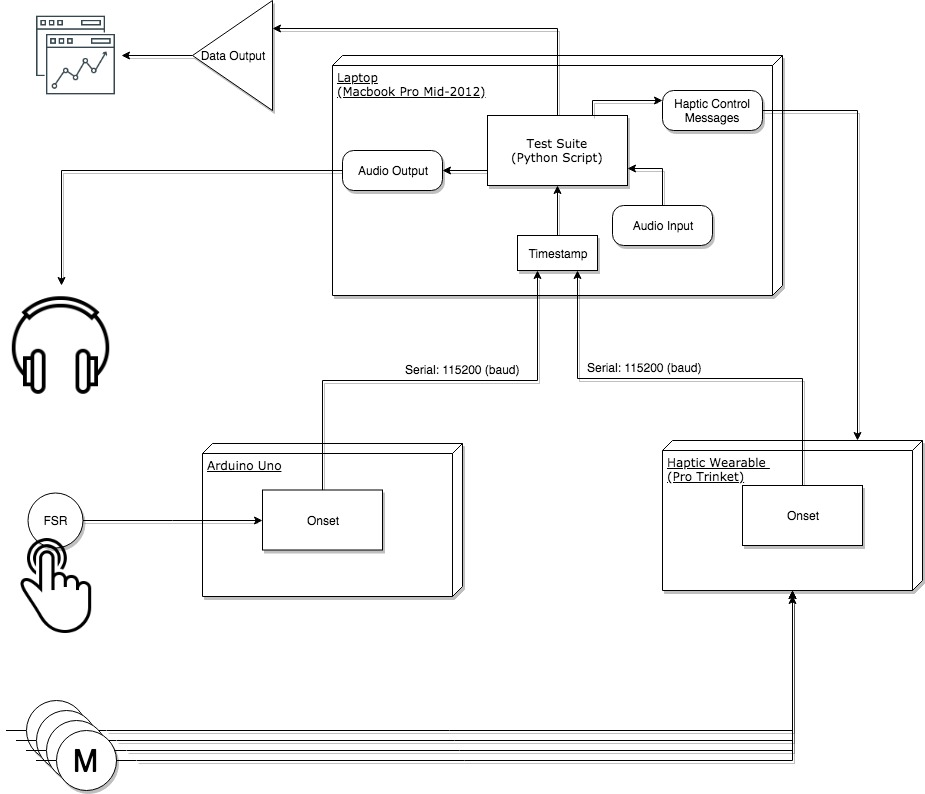
\includegraphics[width=\columnwidth]{TestSuiteFlowDiagram}
    \caption{Test Suite Flow Chart}
    \label{fig:TestSuiteFlowDiagram}
\end{figure}

\subsubsection{Example Output}
    
\section{Expectations}

If it can be proven for nonmusicians that NMA does not exhibit a linear increase as the IOI increases with the haptic...than, x

According to prior research, expect musicians NMAs to be small and nearly constant as IOI is increased.\cite{repp2013sensorimotor,4}



